\documentclass{article}


%% Bring the margins down to 1 inch, like the old ``fullpage'' package.
\usepackage[margin=1.0in]{geometry}

\usepackage{graphicx}
\usepackage{caption}
\usepackage{subcaption}


%% Gives the equivalent of one-and-a-half line spacing.
\linespread{1.3}

\begin{document}

\section{Data description and organization}

Our goal is to estimate the accumulated degree days post mortem based
on the types and prevalences of bacterial and eukaryote organisms
present on pig cadavers.  We made use of the order-level and
family-level taxa which were obtained from 6 pig cadavers over the
course of the study, for which data were collected at intervals during
a period of 61 days.  We decided to focus on the family and order
levels because our early results indicated that analyses at the
phylum-level did not explain nearly as much of the variability as did
models built on family-level and order-level taxa.  At lower even
finer levels (such as genus), we anticipate that an unreasonably large
number of counts would remain unclassified.

Samples were obtained from 6 pig cadavers on 16 different days over
the course of the 61-day period.  Samples were taken more frequently
during the first 15 days (approx.~two weeks) at the beginning of the
study, which is when we would expect rapid changes to occur.  To
account for effect of temperature, we utilized accumulated degree
days, rather than the number of days post mortem.  Table
\ref{tbl:degdays_vs_days} shows all the days on which samples were
taken, along with the corresponding accumulated degree days (ADD).
\begin{table}[hb]
  \centering
  \caption{\label{tbl:degdays_vs_days}Days and accumulated degree days
    (ADD) post mortem}
  \begin{tabular}{r|rrrrrrrrrrrrrrrr}
  Days & 0 & 1 & 2 & 3 & 5 & 7 & 9 & 11 & 13 & 15 & 26 & 33 & 40 & 47 & 54 & 61\\ \hline
  ADD & 0 & 27 & 57 & 87 & 149 & 209 & 267 & 326 & 390 & 448 & 734 & 930 & 1130 & 1326 & 1516 & 1703
  \end{tabular}
\end{table}

Figure \ref{fig:degdays_vs_days} shows that the relationship between
days and ADD is almost linear throughout the study time period.  The
estimated correlation coefficient between calendar days post mortem
and ADD post mortem exceeds 0.99.  This is true when accounting for
the entire time period, or when including only the first 15 days of
observation.
\begin{figure}[hb]
  \centering
  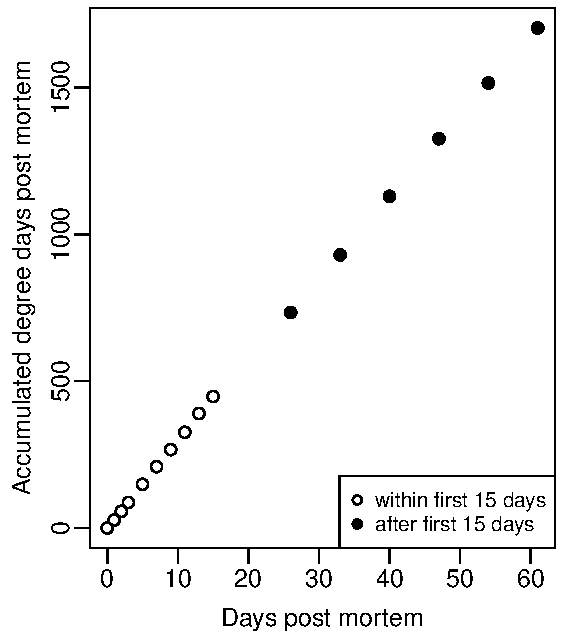
\includegraphics[height=3.5in]{degdays_vs_days}
  \caption{Accumulated degree days vs.~days post mortem}
  \label{fig:degdays_vs_days}
\end{figure}

For the bacterial taxa (Shane's original data), we had to account for
missing data.  Taxa counts were unavailable for subject A1 on days 7
and 9, as well as for subject A4 on day 7.  In addition, the data
collected from subject A3 on day 40 (degree day 1130) is defective.
The total number of taxa (including unclassified taxa) counted for
this cadaver and day was 54.  This is several orders of magnitude less
than the counts for the other cadavers and days, which ranged from
18050 to 93665 (both orders and families).  For this reason, the taxa
from subject A3 on day 40 were omitted.  (Note that the omission of
the A3, day 40 data does not affect the analyses which only consider
the first 15 days of the study.)

Whether working with bacteria or eukaryote data, we did not directly
utilize raw counts in our statistical models.  Exploratory analyses
showed a great deal of variability in the raw counts between
individual cadavers and between days.  Raw counts would also be likely
to vary widely between experiments, which would make our model less
applicable to future experiments.  Instead, we used the proportion of
the counts attributable to each taxa.  First, we excluded all counts
of unclassified taxa from the dataset.  Then, for each taxon, we
calculated the fraction of the counts corresponding to that taxon for
that particular sample (i.e. for that day and for that cadaver).  To
be included in our models, a taxon had to make up at least 1\% of the
daily taxa counts for at least 2 different cadavers, whether on the
same day or on different days.  All taxa which did not meet this
criterion were grouped together as ``rare'' taxa.  This ``rare''
category was not included in our predictive models.  All fractions
attributable to non-rare taxa for individual cadaver and each day were
used as the explanatory variables, while the ADD post mortem
represented the response variable.

While the requirements related to the determination of rare taxa may
seem strange, the idea is to prevent a rare taxon found on just one
cadaver from adversely affecting the model.  In my earlier models
using bacterial family-level taxa, it happened that a particular
taxon, Listeriaceae, that made up more than 1\% of the taxa on only
one cadaver for only one day had been included as an important
predictor in the final model.  My concern is that Listeriaceae may not
be present on future observed cadavers, or, because it is at such low
levels, it may not always be easily measured.  To obtain a more usable
model, I wanted to avoid including taxa which appeared very
infrequently in our samples, or were introduced solely through one
unusual cadaver.


\section{Methods}

Inspired by Metcalf et al.~(2016), we made use of random forest
models.  The random forest methodology is non-parametric, so it does
not depend on distributional assumptions or on finding an mathematical
function to describe an apparent trend or pattern.  It is commonly
used in machine learning applications, since it can be utilized even
when there are a large number of potential explanatory variables and
even when there are dependencies/associations among these explanatory
variables.

A good description of the random forest methodology can be found in
James et al. (2013, Chp.~8).  The approach uses tree-based models to
split the observations into groups, such that at each binary split, we
divide the observations in that tree branch into two groups in which
the variability among the response values in each group is minimized.
To reduce the error associated with this method, we fit multiple trees
(i.e., a ``forest'') using bootstrap samples of the dataset of
interest, with the final model being an average of the ``forest'' of
models.  To reduce the correlation among the trees in the ``forest'',
we consider only a random subset of the potential explanatory
variables at each split.  This is the ``random'' aspect of the
``random forest'' approach.

It is not immediately evident how many explanatory variables should be
considered at each split of the tree, so this number is a parameter
that needs to be estimated.  We use cross-validation to help us choose
this setting for the random forest model, which I called
\texttt{numVarSplit} in my R code.  Another parameter often considered
in random forest models is the number of bootstrapped trees sufficient
for the error to converge to a minimum.  In our cross-validation
studies, 3000 bootstrapped trees appeared to well exceed the number
required, so we used 3000 trees for each model.

To estimate the \texttt{numVarSplit} parameter, I used
cross-validation runs.  For each run, I randomly select a certain
subset (a minority) of the available observations to hold back as a
``validation'' data set.  The rest of the observations make up the
``training'' dataset.  We then fit a series of random forest models on
the training dataset, using a variety of possible values for
\texttt{numVarSplit}.  We then use the models to predict the values
for the validation dataset, and calculate the errors (actual number of
degree days from the validation dataset minus the number of degree
days estimated by the model).  The setting for \texttt{numVarSplit}
which produces the smallest error and the greatest fraction of
variability explained is the one I use for the final model.

As mentioned above, the model fitting procedure depends on the random
selection of which variables to consider at each split of the decision
tree.  Therefore, the final model, using the same data and paramters,
will differ slightly from one to the next or one practitioner to
another.  To get a sense of the variability associated with this
necessary randomness, I fit the final model over and over again, and
looked at how the root mean squared error (RMSE) and the percentage of
explained variance vary.

%%% NEED TO TALK ABOUT THE TWO DIFFERENT SORTS OF CROSS-VALIDATION WE
%%% USED TO TRY TO GET AN IDEA OF LIKELY PERFORMANCE IN PREDICTION
%%% MODE.

I had some concerns about how well our model would perform in
prediction mode.  We have only 6 cadavers, and we only have
observations at certain time steps.  Since our earlier conversation
about our original models, I've reduced the training set to 80\% of
the data, reserving 20\% to use as a test set.  (Previously, the split
was 90\% and 10\%.)  So, when using the bacterial data for all time
steps, this means training on a set of 74 observations, and testing on
a size of 18.  When using just the first 15 days of bacterial data,
this means training on a set of 46 observations, and testing on a size
of 11.  The change from 90\% to 80\% made very little difference in
the choice of models, which relieved some of my concern.  Also, since our
earlier meetings, I figured out how to parallelize some of the
computational work, which allowed me to use some additional
cross-validation runs and to try additional models, compared to what I
had done previously.



\section{Models using all time steps (days 0-61)}


\subsection{Using Shanes's original bacteria data}

We have a total of 92 observations (16 days $\times$ 6 cadavers, minus
the 4 missing cadaver-day combinations mentioned in the data
description section).  Across all days and cadavers, about 29.3\% of
the taxa were ``unclassified''.  There were 39 family-level taxa
considered as potential predictors, when doing analyses for the whole
time period.

Figure \ref{fig:infl_bac_family_taxa} shows measures of model
importance for the 6 most influential taxa.  (I have chosen 6
simply because it's easy to show a 2 by 3 panel of plots.  If we
display more, it tends to be too much information to easily digest.)
The measure of importance is the mean percentage increase in the
mean-square error of model predictions, when we consider models in
which the variable in question is left out of the model.  It should be
noted that this measure is one of the two commonly used methods for
measuring the importance of the individual taxa; the other measure,
called ``node purity'', is harder to explain.  These meaures do
sometimes differ on the ranking of taxa influence, as there is more
than one way to judge the relevance of a particular predictor.
However, in the course of doing these analyses, I've noticed that both
measures generally feature the same important taxa, though their
relative rankings may be different.
\begin{figure}
  \centering
  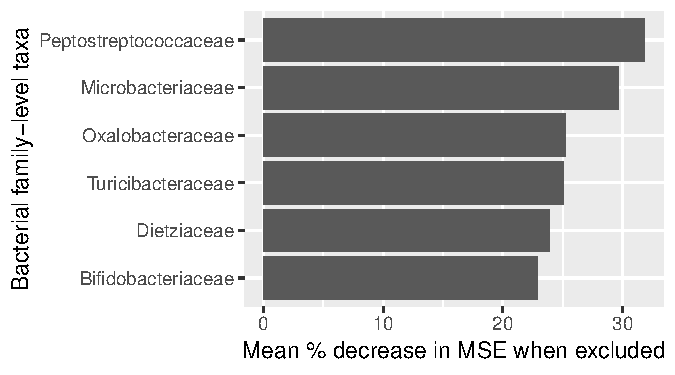
\includegraphics[width=4in]{../revise_algorithm/only_families/all_time_steps/hit_1perc_twice/orig_units_all_data_families_PercIncMSE_barchart}
  \caption{Most influential bacterial family-level taxa (all time steps)}
  \label{fig:infl_bac_family_taxa}
\end{figure}

Figure \ref{fig:infl_bac_family_scatter} provides scatterplots
corresponding to these six taxa.  Each point in the plots below
corresponds to the measured fraction of classified bacteria belonging
to the designated taxa on each of the degree days.  Note that the
scales of the vertical axes differ among the taxa.
\begin{figure}
  \centering
  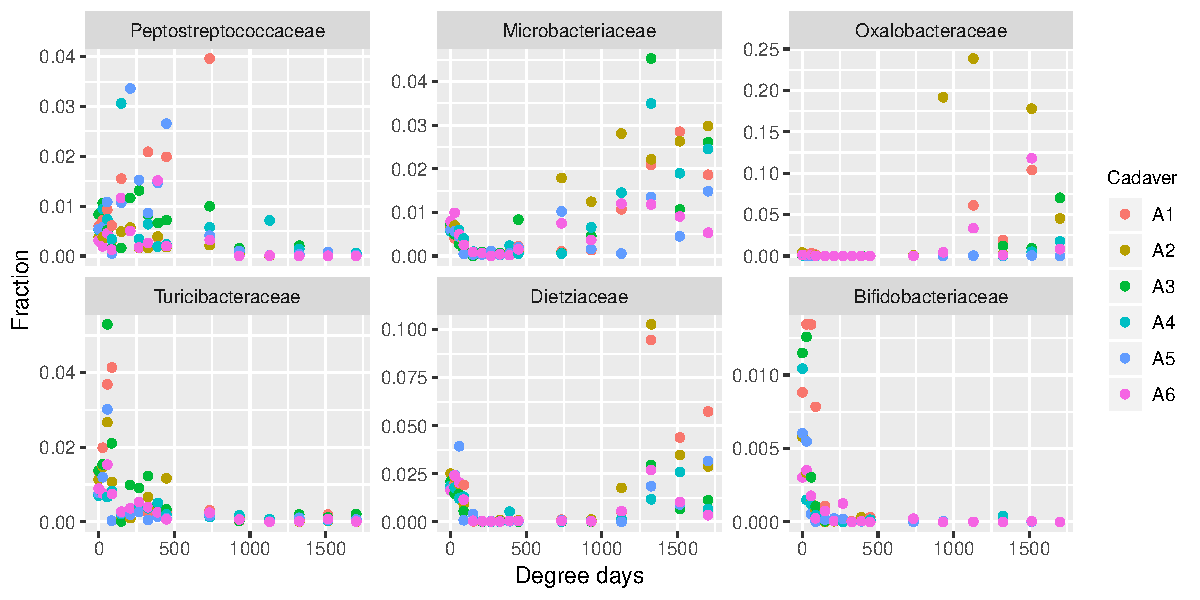
\includegraphics[width=7.5in]{../revise_algorithm/only_families/all_time_steps/hit_1perc_twice/infl_bac_family_all_data_scatter}
  \caption{Scatterplots for influential bacterial family-level taxa (all time steps)}
  \label{fig:infl_bac_family_scatter}
\end{figure}

\begin{table}
  \centering
\caption{\label{tbl:final_model_stats_all_days}Final model statistics using family-level taxa, all time steps}
\begin{tabular}{llrr}
Source data & Level & RMSE (using all data) & Explained variation (using all data)\\ \hline %% & RMSE (cross-valid. mirroring real-life)\\ \hline
Bacteria  & Family-level & 208 ($\pm$ 3) & 85.9\% ($\pm$ 0.4\%)\\ %%& 274.8\\
%% Bacteria  & Family-level & 207.2 & 86.1\% & 274.8\\
%% Eukaryote & Family-level & 178.1 & 89.5\% & 243.6 %%\\
\end{tabular}
\end{table}

To get an idea of the errors (also called residuals) associated with
the random forest model, I did 1000 additional cross-validation runs,
using a random forest model with the optimal value of the variable
\texttt{numVarSplit} determined through the initial set of
cross-validation runs.  The cross-validations are done by randomly
choosing 20\% of the dataset to leave out the model-fitting procedure.
Then, the model (fitted on the remaining 80\%) is used to estimate the
responses for the observations that were left out.  Figure
\ref{fig:resids_cv_bac_family_taxa} illustrates the model errors
(actual minus estimated) vs.~the actual values, taken across these
1000 cross-validation runs.  \textbf{Next sentence not currently
  true.}  The RMSE for these runs is given in the random
cross-validation column in Table
\ref{tbl:family_all_data_model_stats}.  For the beginning of the time
period (lower degree days), the model is over-predicting, while the
opposite is true at the end of the time period.  The model estimates
are biased toward the average degree day.  This error pattern looks
similar to that in Figure S9 in the Metcalf et al. (2015)
supplementary material.

\begin{table}
  \centering
\caption{\label{tbl:valid_model_stats_all_days}Cross-validation statistics using family-level taxa, all time steps}
\begin{tabular}{llrr}
Source data & Level & RMSE (random) & RMSE (leave out 1 subj., 1 day)\\ \hline
Bacteria  & Family-level & 219 ($\pm$ 78) & 227 ($\pm$ 106)\\ %%& 274.8\\
%% Bacteria  & Family-level & 207.2 & 86.1\% & 274.8\\
%% Eukaryote & Family-level & 178.1 & 89.5\% & 243.6 %%\\
\end{tabular}
\end{table}


\begin{figure}
  \centering
  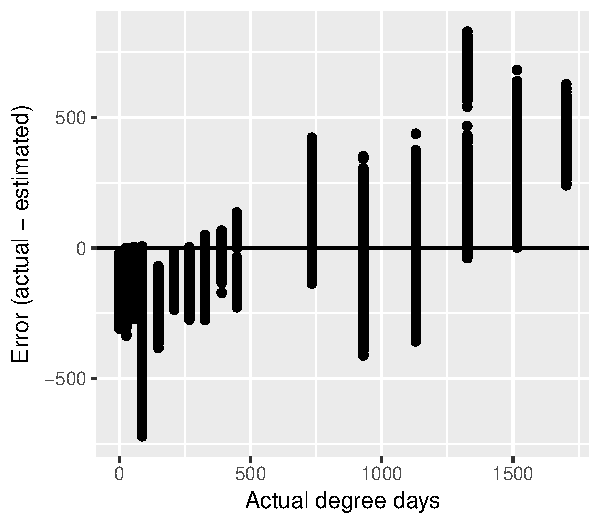
\includegraphics{../revise_algorithm/only_families/all_time_steps/hit_1perc_twice/orig_units_all_data_families_residuals}
  \caption{Residuals from the cross-validation runs for the bacterial
    family-level taxa model}
  \label{fig:resids_cv_bac_family_taxa}
\end{figure}

One of my concerns is that while the cross-validation described above
is good way to assess a model's performance, this traditional approach
does not quite reflect the particular issues involved in how we would
realistically use this model.  In practice, we would be using this
model to predict the ADD post mortem based on the counts of
family-level taxa from a never-before-observed cadaver.  The actual
post mortem interval in such a case would be unlikely to correspond
with a number of accumulated degree days which we have previously
observed in our experiments.  For instance, we might be dealing with a
cadaver for which the interval post mortem is actually 100 or 500 ADD.
To get a better idea about how the model might be expected to perform
in such a situation, we fit the model for 96 (16 days $\times$ 6
cadavers) particular cross-validation sets.  For each set, we leave
out all the observations associated with one particular cadaver (on
any day) and all the observations associated with one accumulated
degree day (for any cadaver).  Then, we calculate the prediction
errors for the left-out cadaver on the left-out day.

Figure \ref{fig:leave_one_out_resids_bac_family_taxa} shows the
residuals for all combinations of degree day and subject.  The RMSE
for these runs is about 274.8, which is higher than the RMSE for the
model including all data, which is given in Table
\ref{tbl:family_all_data_model_stats}.  This larger error stems from
two sources.  First, Table \ref{tbl:family_all_data_model_stats} shows
the model performance statistics based on fitting the model with all
available data, while these runs purposefully left out all the data
for a certain subject and for a certain day.  Second, by construction,
these test runs were conducted while omitting all information about a
particular degree day, so that there is a gap in the information
available.  In contrast, the RMSE associated with estimates for
left-out subjects on days that were not left out is only about 220.9.

\begin{figure}
  \centering
  \includegraphics{../revise_algorithm/only_families/all_time_steps/hit_1perc_twice/leave_out_one_subj_and_one_day_residuals}
  \caption{Residuals for model runs leaving out one subject and one day (bacterial family-level taxa)}
  \label{fig:leave_one_out_resids_bac_family_taxa}
\end{figure}


\subsection{Using Luisa's eukaryote data}

In the eukaryote data, we don't have missing data for any day-subject
combinations.  Therefore, we have a total of 96 observations (16 days
$\times$ 6 cadavers), which is 4 more observations than were available
with the bacterial data.  Across all days and cadavers, about 32.76\%
of the taxa were unclassified.  As before, ``unclassified'' counts
were excluded from the analysis.  There were 39 family-level taxa
considered as potential predictors when doing analyses for the entire
time period.

Figure \ref{fig:infl_euk_family_taxa} shows measures of model
importance for the most influential eukaryotic family-level taxa.  The
measure of importance is the same used for the bacteria family-level
taxa, as in Figure \ref{fig:infl_bac_family_taxa}.  These same taxa
are featured in Figure \ref{fig:infl_euk_family_all_data_scatter},
which shows how the fraction of counts attributed to them change over
the time period and across individual cadavers.
\begin{figure}
  \centering
  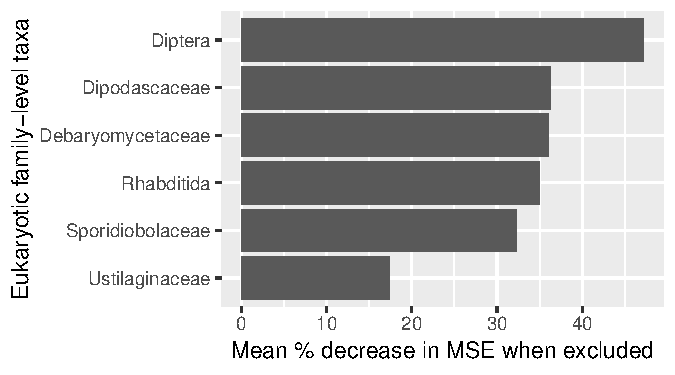
\includegraphics{../eukaryote_data/only_families/all_time_steps/hit_1perc_twice/orig_units_all_data_families_PercIncMSE_barchart}
  \caption{Most influential eukaryotic family-level taxa (all time steps)}
  \label{fig:infl_euk_family_taxa}
\end{figure}

\begin{figure}
  \centering
  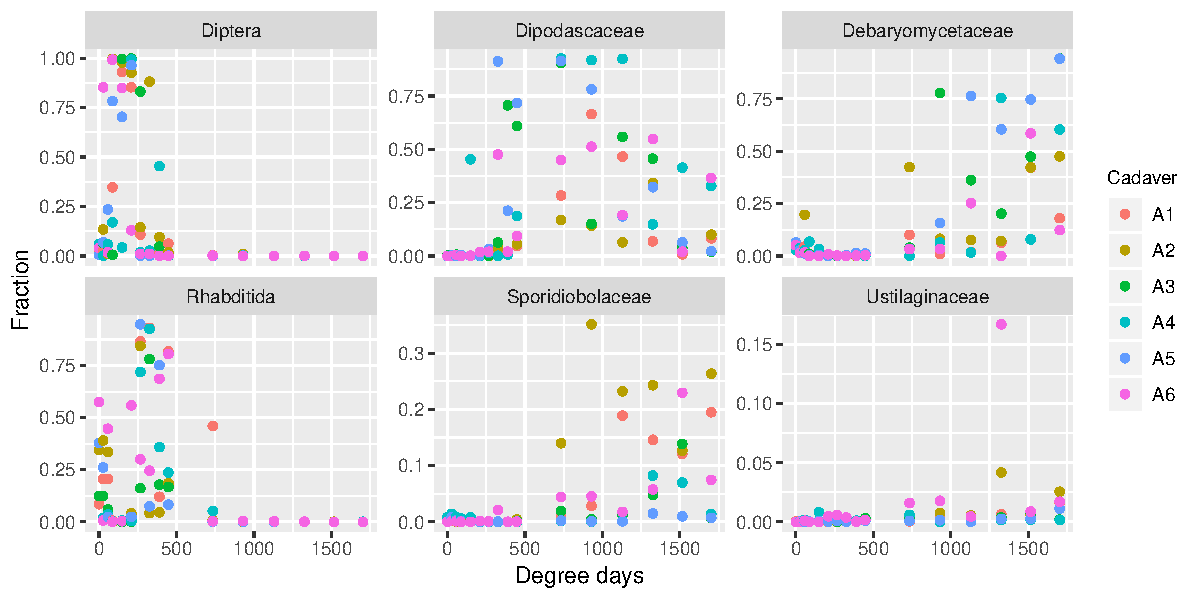
\includegraphics[width=7.5in]{../eukaryote_data/only_families/all_time_steps/hit_1perc_twice/infl_euk_family_all_data_scatter}
  \caption{Scatterplots for influential eukaryotic family-level taxa (all time steps)}
  \label{fig:infl_euk_family_all_data_scatter}
\end{figure}

The final model using the eukaryote data is a better fit than that
using the bacteria data, as shown in the model performance statistics
featured in Table \ref{tbl:family_all_data_model_stats}.  The RMSE is
about 178.1, which is about 30 ADD less than that for the bacterial
data.  When we look at the more ``real-life'' cross-validation study
(leaving out all data associated with one combination of subject and
day, in turn), the cross-validation RMSE is about 243.6, which is also
substantially less than that for the bacterial ``real-life''
cross-validation tests.




\section{Models using only the first 15 days of the study period}

\subsection{Using Shanes's original bacteria data}

For the analyses considering the first 15 days (approximately two
weeks), we have 57 observations.  These represent observations on 6
cadavers on 10 observation days, minus the 3 missing cadaver-day
combinations occurring during this period.  This includes the missing
data for subject A1 on days 7 and 9 and the missing data for subject
A4 on day 7 of the study.

Figure \ref{fig:infl_bac_first_15_days_family_taxa} shows the taxa
considered most important in the model fitting process.  We note that
the top four taxa are different between the model using all the data
(as shown in Figure \ref{fig:infl_bac_family_taxa}) and this model
focused on the first couple of weeks.  The ``top four'' consist of
Flavobacteriaceae, Lactobacillaceae, Pseudomonadaceae, and
Dermabacteraceae, none of which entered the top eight of the model
using all the time steps.  The scatterplots for these taxa, for the
first 15 days of the time period, are shown in Figure
\ref{fig:infl_bac_first_15_days_family_scatter}.
\begin{figure}
  \centering
  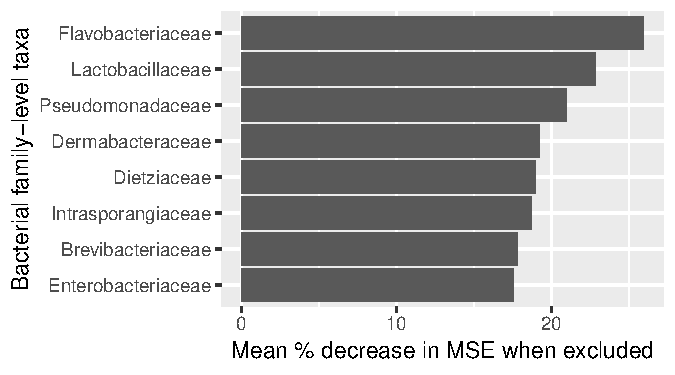
\includegraphics[width=4in]{../revise_algorithm/only_families/first_two_weeks/hit_1perc_twice/orig_units_first_two_weeks_families_PercIncMSE_barchart}
  \caption{Most influential bacterial family-level taxa (first 15 days)}
  \label{fig:infl_bac_first_15_days_family_taxa}
\end{figure}
\begin{figure}
  \centering
  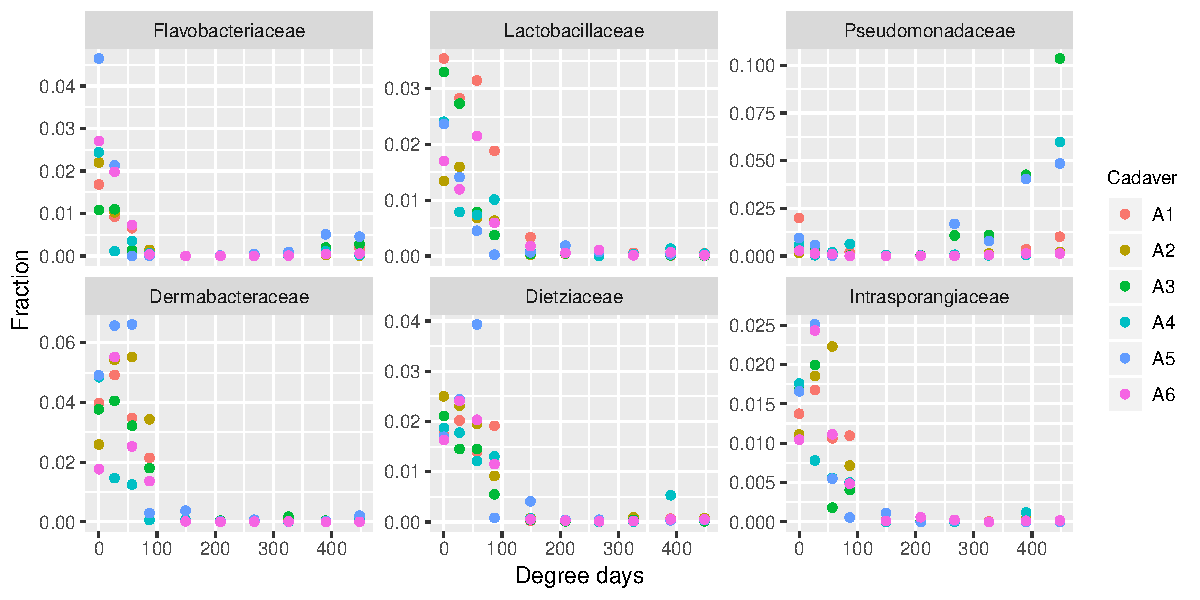
\includegraphics[width=7.5in]{../revise_algorithm/only_families/first_two_weeks/hit_1perc_twice/infl_bac_family_first_two_weeks_scatter}
  \caption{Scatterplots for influential bacterial family-level taxa (first two weeks)}
  \label{fig:infl_bac_first_15_days_family_scatter}
\end{figure}


\begin{table}
  \centering
\caption{\label{tbl:family_first_two_weeks_model_stats}Model statistics using family-level taxa, first 15 days}
\begin{tabular}{ccccc}
Source data & Level & RMSE (all data) & Explained variation & RMSE (as likely used)\\ \hline
Bacteria  & Family-level & 64.3 & 82.4\% & 83.5\\
Eukaryote & Family-level & 58.6 & 84.6\% & 93.1 %%\\
\end{tabular}
\end{table}



\subsection{Using Luisa's eukaryote data}

\begin{figure}
  \centering
  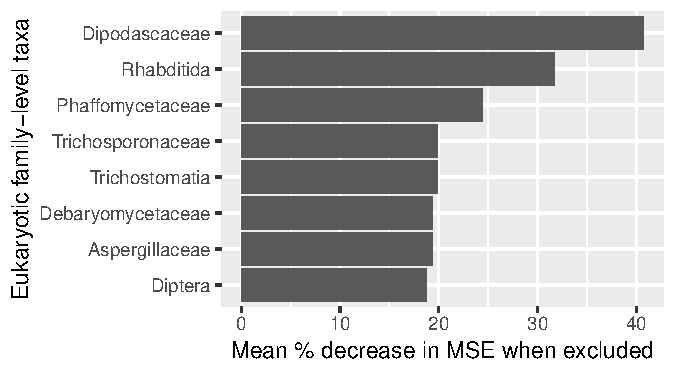
\includegraphics[width=4in]{../eukaryote_data/only_families/first_two_weeks/hit_1perc_twice/orig_units_first_two_weeks_families_PercIncMSE_barchart}
  \caption{Most influential eukaryotic family-level taxa (first 15 days)}
  \label{fig:infl_euk_first_15_days_family_taxa}
\end{figure}
\begin{figure}
  \centering
  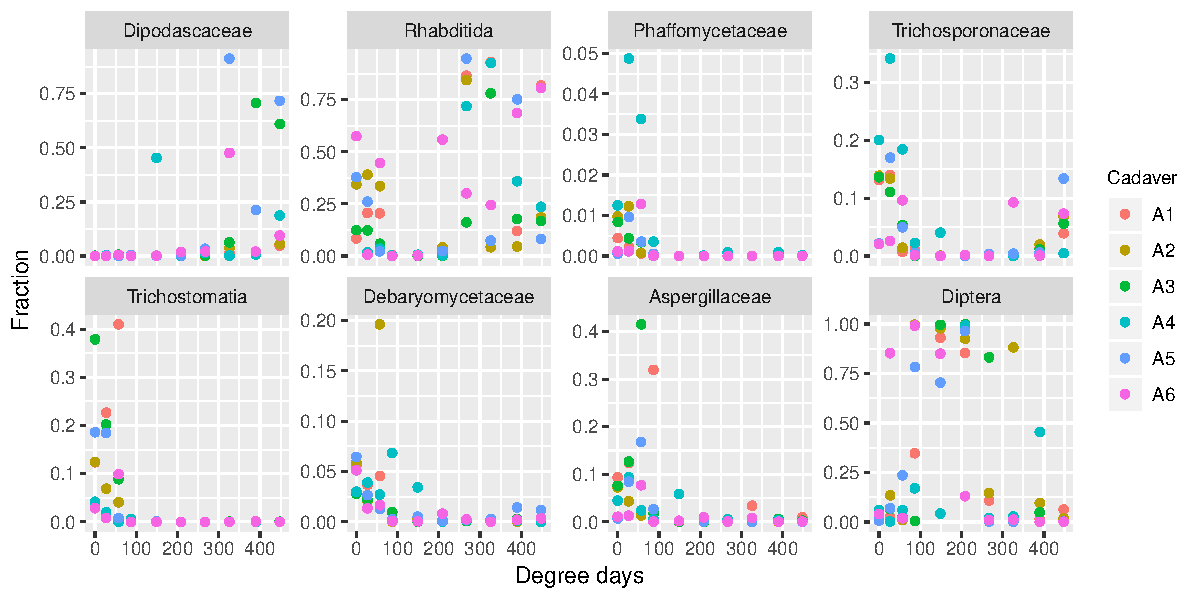
\includegraphics[width=7.5in]{../eukaryote_data/only_families/first_two_weeks/hit_1perc_twice/infl_euk_family_first_two_weeks_scatter}
  \caption{Scatterplots for influential eukaryotic family-level taxa (first two weeks)}
  \label{fig:infl_euk_first_15_days_family_scatter}
\end{figure}




\section{References}

\noindent James, G., Witten, D., Hastie, T., Tibshirani, R. (2013) \textit{An
  Introduction to Statistical Learning with Applications in R}. New
York: Springer

\noindent Metcalf, J. L., et al. (2016).  Microbial community assembly and
metabolic function during mammalian corpse decomposition.
\textit{Science}, Vol.~351, 158-162.


\end{document}







\subsection{Models using all time steps}

In this section, we utilize data collected on all available days.  The
number of days post mortem, along with the corresponding accumulated
degree days, are shown below.

\begin{center}
\begin{tabular}{r|rrrrrrrrrrrrrrrr}
  Day & 0 & 1 & 2 & 3 & 5 & 7 & 9 & 11 & 13 & 15 & 26 & 33 & 40 & 47 & 54 & 61\\
  Degree day & 0 & 27 & 57 & 87 & 149 & 209 & 267 & 326 & 390 & 448 & 734 & 930 & 1130 & 1326 & 1516 & 1703
\end{tabular}
\end{center}



\subsubsection{Results for family-level taxa}

In our original analysis, we excluded from the model any taxa which
made up less than 1\% of the observed taxa for all cadavers and all
days.  That is, in order to be included, a particular family-level
taxa had to make up at least 1\% of the counts on just one day for
just one individual.  This has the advantage of being an easy cutoff
to implement and to explain.  However, this means that a taxa can be
included based on one unusual observation, even if this taxa is rarely
observed in the vast majority of cases.

To address these concerns, I also ran the analyses with a stricter
cutoff criterion.  Now, in order to be considered in the random forest
model, a taxa must make up more at least 1\% of the counts for at
least two separate cadavers.  These exceedances can happen on the same
day or on different days.  This addresses the concern that one
particularly unusual cadaver can cause taxa to be considered in the
model which are not generally present on other cadavers.  It also
makes explaining the model a bit easier, because there are fewer taxa
to consider and outlying taxa are less likely to affect the fit.

To illustrate the differences, consider the analysis using
family-level taxa for all time steps.  Using the original cutoff
criterion, the model considers 49 possible family-level taxa.  The
most influential taxa identified by the resulting model are shown in
Figure \ref{fig:infl_family_taxa_orig_crit}.  Their influence on the
model is determined by how much the node impurity (i.e., the
variability in the ``leaves'' of the decision tree) is reduced by
including these particular family-level taxa in the random forest
model.  That is, a more influential taxa is associated with a large
decrease in this variability.

\begin{figure}
  \centering
  \includegraphics{../../only_families/all_time_steps/cutoff_1perc/orig_units_all_data_families_barchart}
  \caption{Most influential family-level taxa, modeled using a weak inclusion criterion}
  \label{fig:infl_family_taxa_orig_crit}
\end{figure}


When using the original cutoff, the algorithm picks the Listeriaceae
family as an important predictor.  However, the the Listeriaceae
family exceeds 1\% of the total counts for only one day and one
individual.  Figure \ref{fig:scatter_family_taxa} shows some of the
influential families by degree day.  Note the varying scales on the
vertical axes.  We see that the Listeriaceae family only exceeds 1\%
of the total counts on one degree day (1516) for one subject.  So, my
concern is that Listeriaceae may not be present on future observed
cadavers, or, because it is at such low levels, it may not always be
easily measured.

\begin{figure}
  \centering
  \includegraphics{../../only_families/all_time_steps/influential_family_taxa_panel}
  \caption{Some of the influential family-level taxa, by degree day}
  \label{fig:scatter_family_taxa}
\end{figure}

Figure \ref{fig:infl_family_taxa_stric_crit} shows the same type of
plot, but for the random forest model developed using the stricter
criterion.  Again, this criterion only allows taxa to be included if
the taxa makes up at least 1\% of the total counts for at least two
cadavers (can be on same or different days).  Therefore, this stricter
cutoff excludes Listeriaceae, and allows fewer (39) family-level taxa
to be included in the model.  Even so, the statistics presented in
Table \ref{tbl:family_all_data_model_stats} indicates that the
explanatory value of this model is almost as strong.

\begin{figure}
  \centering
  \includegraphics{../../only_families/all_time_steps/hit_1perc_twice/orig_units_all_data_families_barchart}
  \caption{Most influential family-level taxa, modeled using a stricter inclusion criterion}
  \label{fig:infl_family_taxa_stric_crit}
\end{figure}


\begin{table}
  \centering
\caption{\label{tbl:family_all_data_model_stats}Model statistics using family-level taxa}
\begin{tabular}{llll}
Inclusion cutoff & Units  & RMSE & Explained variation\\ \hline
1\% at least once (weaker)  & Orig.~units & 198.58 & 87.21\%\\
1\% at least twice (stricter) & Orig.~units & 207.18 & 86.08\% %%\\
%% 1\% at least once  & Sqrt.~units & 4.18 & 88.70\%\\
%% Didn't do the sqrt runs with the stricter cutoff.
\end{tabular}
\end{table}

To get an idea of the errors (also called residuals) made by the
random forest model, I used cross-validation runs.  Remember, the
cross-validations are done by randomly choosing 20\% of the dataset to
leave out the model-fitting procedure.  Then, the model (fitted on the
remaining 80\%) is used to estimate the responses for the observations
that were left out.  Figure \ref{fig:resids_cv_family_taxa}
illustrates the model errors (actual minus estimated) vs.~the actual
values, taken across 1000 cross-validation runs.  For the beginning of
the time period (lower degree days), the model is over-predicting,
while the opposite is true at the end of the time period.  The model
estimates are biased toward the average degree day.

\begin{figure}
  \centering
  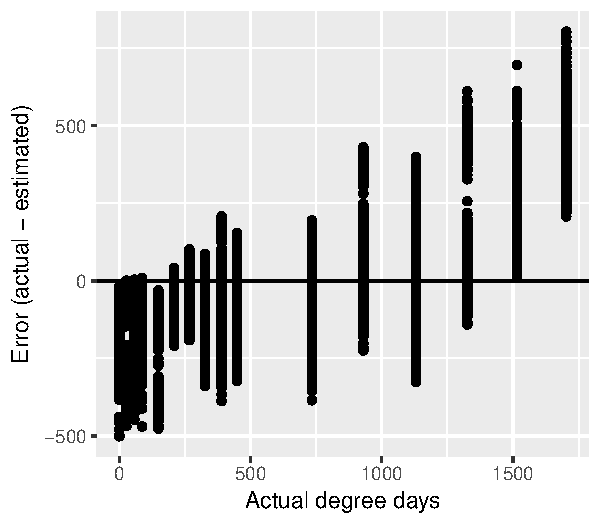
\includegraphics{../../only_families/all_time_steps/hit_1perc_twice/orig_units_all_data_families_residuals}
  \caption{Residuals from the cross-validation runs for the family taxa model}
  \label{fig:resids_cv_family_taxa}
\end{figure}

In practice, we would be using this model to predict the accumulated
degree days based on the counts of family-level taxa from a never
before observed cadaver.  The post mortem interval in such a case
would not necessarily correspond with a number of accumulated degree
days which we have observed before.  For instance, we might observe a
cadaver at a time associated with 100 degree days or 500 degree days.
To get a better idea about how the model might be expected to perform
in such a situation, we fit the model 96 times, leaving one subject
and one degree day out each time (16 degree days X 6 subjects).  Then,
we calculate the errors in the model estimates made for the subject
which was left out on the day which was left out.

Figure \ref{fig:leave_one_out_resids_family_taxa} shows the residuals
for all combinations of degree day and subject.  The RMSE for these
runs is about 274.8, which is higher than the RMSE for the model
including all data, which is given in Table
\ref{tbl:family_all_data_model_stats}.  This larger error stems from
two sources.  First, Table \ref{tbl:family_all_data_model_stats} shows
the model performance statistics based on fitting the model with all
available data, while these runs purposefully left out all the data
for a certain subject and for a certain day.  Second, by construction,
these test runs were conducted while omitting all information about a
particular degree day, so that there is a gap in the information
available.  In contrast, the RMSE associated with estimates for
left-out subjects on days that were not left out is only about 220.9

\begin{figure}
  \centering
  \includegraphics{../../only_families/all_time_steps/hit_1perc_twice/leave_out_one_subj_and_one_day_residuals}
  \caption{Residuals for model runs leaving out one subject and one day (family-level taxa)}
  \label{fig:leave_one_out_resids_family_taxa}
\end{figure}




\subsubsection{Results for order-level taxa}

For the order-level taxa, I also ran the analysis both ways, with the
stricter inclusion criterion (requiring 1\% for at least two cadavers)
and the weaker, original one.  Again, the model performance is similar
for both, so I think we should go with the stricter cutoff.  With the
stricter cutoff, the model considers 15 order-level taxa, versus 20
taxa with the original criterion.  The relevant performance statistics
are given in Table \ref{tbl:order_all_data_model_stats}.

\begin{table}
  \centering
  \caption{\label{tbl:order_all_data_model_stats}Model statistics using order-level taxa}
\begin{tabular}{llll}
Inclusion cutoff & Units  & RMSE & Explained variation\\ \hline
1\% at least once (weaker)  & Orig.~units & 230.19 & 82.81\%\\
1\% at least twice (stricter) & Orig.~units & 230.65 & 82.74\%
%% 1\% at least once  & Sqrt.~units &   4.38 & 87.62\%\\
%% Didn't do the sqrt runs with the stricter cutoff.
\end{tabular}
\end{table}

Figure \ref{fig:infl_order_taxa_stric_crit} shows the orders found
to be most influential in building the random forest model using the
stricter inclusion criterion.  These are similar to those found
previously, using the weaker inclusion criterion, with the one
noticeable difference being the elimination of the Bifidobacteriales
order.  This order exceeded 1\% of the total counts for only one
cadaver, so it could not be considered under the stricter inclusion
criterion.  Figure \ref{fig:scatter_order_taxa} shows the fraction of
counts associated with the six order taxa that were most influential
in the order-level random forest model.  Again, note the varying
scales of the y-axes across the panels.  The error patterns for the
models using order-level taxa are very similar to those for the
family-level taxa, so I haven't included them here.

\begin{figure}
  \centering
  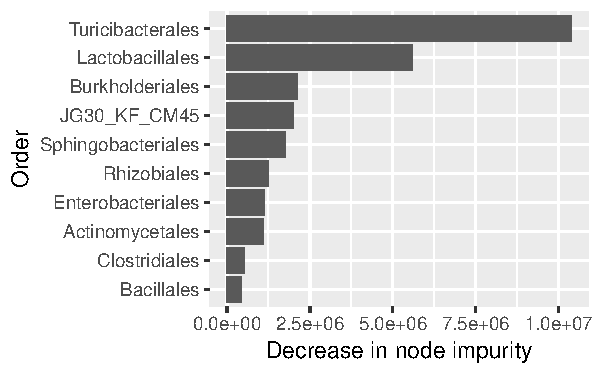
\includegraphics{../../only_orders/all_time_steps/hit_1perc_twice/orig_units_all_data_orders_barchart}
  \caption{Most influential order-level taxa, modeled using a stricter inclusion criterion}
  \label{fig:infl_order_taxa_stric_crit}
\end{figure}


\begin{figure}
  \centering
  \includegraphics{../../only_orders/all_time_steps/influential_order_taxa_panel}
  \caption{Some of the influential order-level taxa, by degree day}
  \label{fig:scatter_order_taxa}
\end{figure}



\subsection{Models using only the first 15 days of data}

\subsubsection{Results for family-level taxa}

Table \ref{tbl:family_first_15days_model_stats} shows the model
performance statistics for the model using just the first 15 days of
family-level taxa.  Whether we use the weaker or stronger inclusion
criteria, model performance is much the same, so we go with the
stricter criterion for each of interpretation and implementation.  For
the first 15 days of data, we consider 35 possible family-level taxa.
As we might expect, the influential taxa for this early period are
different than those for the full time period.  The top 10 such taxa
are shown in Figure
\ref{fig:infl_family_taxa_first_15days_stric_crit}.  Scatterplots of
six of these taxa are found in Figure
\ref{fig:scatter_family_taxa_first_15days}.  Again, note the
difference in scaling of the y-axis among the various panels.

\begin{table}
  \centering
  \caption{\label{tbl:family_first_15days_model_stats}Model statistics using family-level taxa for the first 15 days}
\begin{tabular}{llll}
Inclusion cutoff & Units  & RMSE & Explained variation\\ \hline
1\% at least once (weaker) & Orig.~units & 64.98 & 81.99\%\\
1\% at least twice (stricter) & Orig.~units & 64.25 & 82.39\%
%% 1\% at least once  & Sqrt.~units & 2.31 & 87.87\%\\
%% 1\% at least twice & Sqrt.~units & 2.28 & 88.20\%
\end{tabular}
\end{table}

\begin{figure}
  \centering
  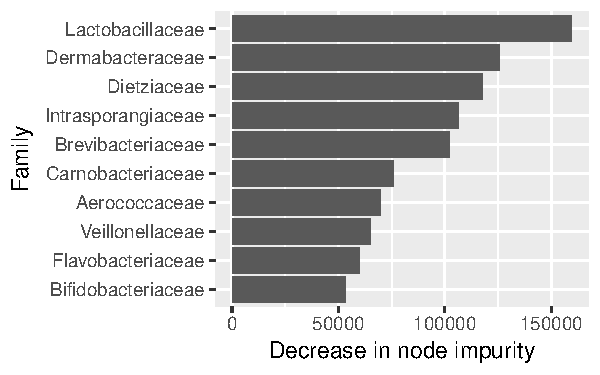
\includegraphics{../../only_families/first_two_weeks/hit_1perc_twice/orig_units_first_two_weeks_families_barchart}
  \caption{Most influential family-level taxa in the first 15 days, modeled using a stricter inclusion criterion}
  \label{fig:infl_family_taxa_first_15days_stric_crit}
\end{figure}

\begin{figure}
  \centering
  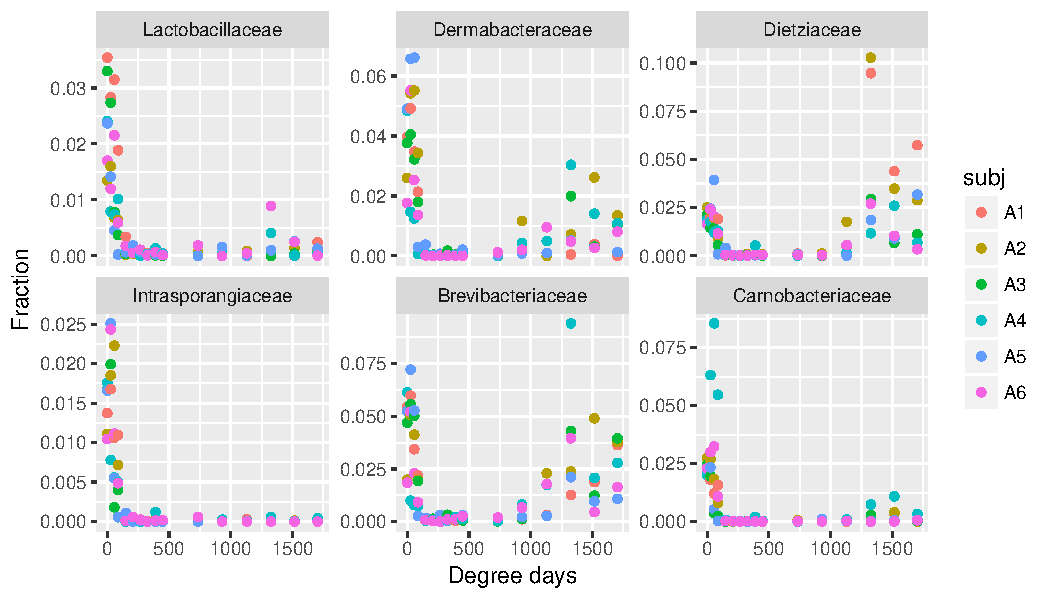
\includegraphics{../../only_families/first_two_weeks/influential_family_taxa_panel_first_two_weeks}
  \caption{Some of the influential family-level taxa, for the first 15 days}
  \label{fig:scatter_family_taxa_first_15days}
\end{figure}

Looking at the residuals, we see the same patterns that we saw for the
model using all time steps.  Figure
\ref{fig:resids_cv_first_15days_family_taxa} shows the errors
associated with 1000 cross-validation runs, with the training and
validation sets selected randomly.  However, since the analysis is
limited to the first two weeks, the RMSE is correspondingly lower.

\begin{figure}
  \centering
  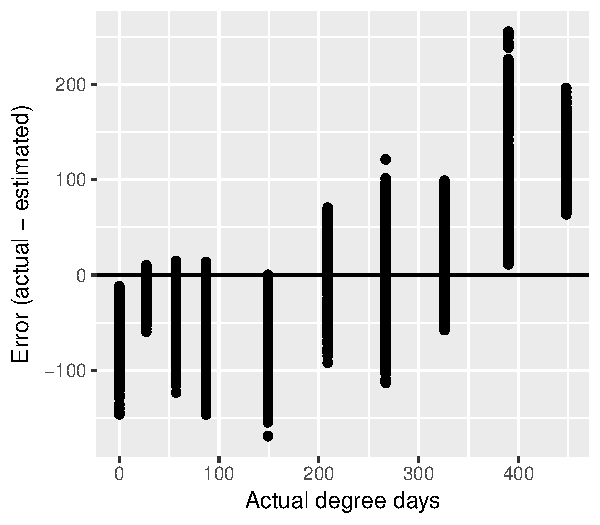
\includegraphics{../../only_families/first_two_weeks/hit_1perc_twice/orig_units_first_two_weeks_families_residuals}
  \caption{Residuals from the cross-validation runs for the family taxa model, first 15 days}
  \label{fig:resids_cv_first_15days_family_taxa}
\end{figure}

Figure \ref{fig:leave_out_one_resids_family_taxa_first_15days} shows
the residuals when we each combination of one subject and one time
step out of the model-fitting process.  Again, this is very similar to
the pattern we saw when using the data from the whole time period.
The RMSE for these runs is about 83.5.  This means that in a real-life
situation, in which it's likely that we do not have observations from
the applicable degree day, the RMSE is substantially higher than the
RMSE for the fitted model.
%% The RMSE for situations where we are predicting the left-out
%% individual for days which are present in the model is about 66.1.

\begin{figure}
  \centering
  \includegraphics{../../only_families/first_two_weeks/hit_1perc_twice/leave_out_one_subj_and_one_day_residuals}
  \caption{Residuals for model runs leaving out one subject and one day, first 15 days (family-level taxa)}
  \label{fig:leave_out_one_resids_family_taxa_first_15days}
\end{figure}


\subsubsection{Results for order-level taxa}

Looking at the model for the first 15 days, using the order-level
taxa, the models with the stricter and weaker inclusion cutoffs are
again very similar.  The model performance statistics are shown in the
Table \ref{tbl:order_first_15days_model_stats}.  We stick with the
stricter inclusion criterion, which utilizes 14 orders in the random
forest model.  Figure
\ref{fig:infl_order_taxa_first_15days_stric_crit} shows the 10 most
influential order-level taxa in the model, and Figure
\ref{fig:scatter_order_taxa_first_15days} provides a sense of how the
fractions attributable to six of these taxa are changing over the
first 15 days.

\begin{table}
  \centering
  \caption{\label{tbl:order_first_15days_model_stats}Model statistics using order-level taxa for the first 15 days}
\begin{tabular}{llll}
Inclusion cutoff & Units  & RMSE & Explained variation\\ \hline
1\% at least once (weaker) & Orig.~units & 53.93 & 87.59\%\\
1\% at least twice (stricter) & Orig.~units & 54.68 & 87.25\%
%% 1\% at least once  & Sqrt.~units & 2.01 & 90.81\%
%% 1\% at least twice & Sqrt.~units & 2.02 & 90.68\%
\end{tabular}
\end{table}

\begin{figure}
  \centering
  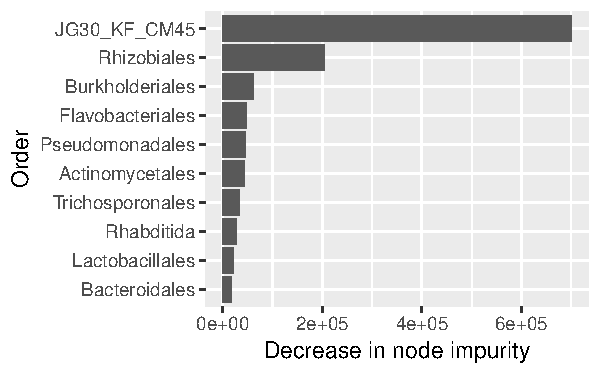
\includegraphics{../../only_orders/first_two_weeks/hit_1perc_twice/orig_units_first_two_weeks_orders_barchart}
  \caption{Most influential order-level taxa in the first 15 days, modeled using a stricter inclusion criterion}
  \label{fig:infl_order_taxa_first_15days_stric_crit}
\end{figure}

\begin{figure}
  \centering
  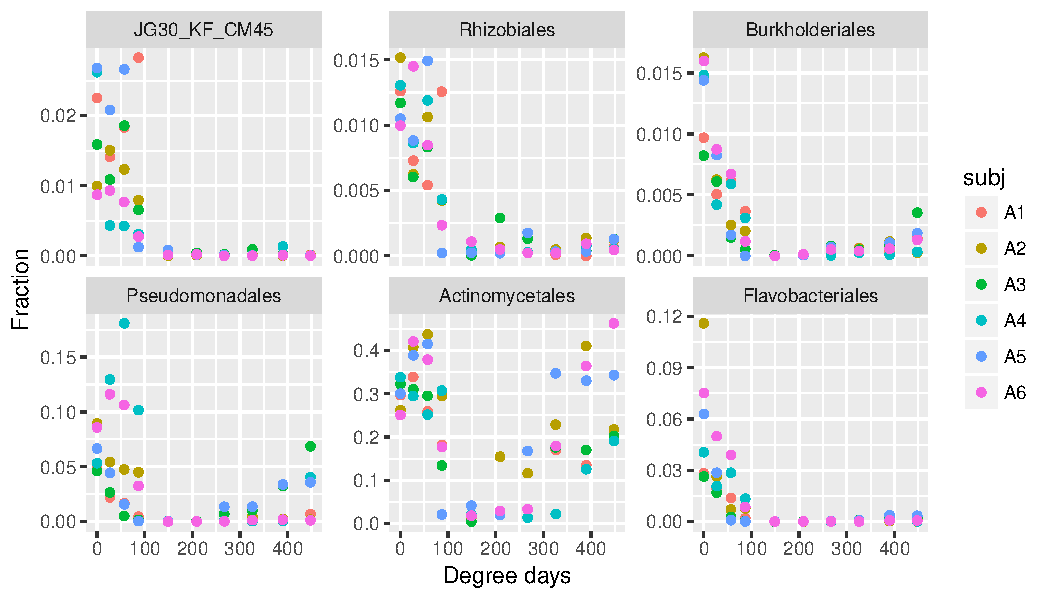
\includegraphics{../../only_orders/first_two_weeks/influential_order_taxa_panel_first_two_weeks}
  \caption{Some of the influential order-level taxa, for the first 15 days}
  \label{fig:scatter_order_taxa_first_15days}
\end{figure}


\section{Working with Luisa's eukaryote data}

\subsection{Overview}

I applied the same methods to Luisa's eukaryote data, again focusing
on family-level and order-level taxa.  I did not find any day/subject
combination with an unusually low count, as I did for subject A3 on
day 40 of Shane's data.  However, I did find very small numbers of
counts from orders Mammalia and Aves, which I excluded from the
analysis.

The cross-validation procedures I used were also the same as those
used previously.  I focused on the stricter inclusion criterion,
meaning that, for inclusion in the analysis, a taxon must make up more
than 1\% of the total daily counts on at least 2 cadavers.  Again,
this reduces the number of taxa to consider, and hopefully makes the
analysis more resistant to outliers and easier to implement in a
real-life estimation.

\subsection{Models using all time steps}

\subsubsection{Results for family-level taxa}

The model statistics for the final random forest model, using both the
weaker and stronger inclusion criteria, are found in Table
\ref{tbl:eukaryote_family_all_data_model_stats}.  As before, the
goodness-of-fit is very similar, so for the remainder of the analyses,
I will stick with models following the stricter criterion.  Note that
this model seems to fit better than the model making use of the
previous bacteria-only dataset.

\begin{table}
  \centering
\caption{\label{tbl:eukaryote_family_all_data_model_stats}Model statistics using family-level eukaryote taxa}
\begin{tabular}{llll}
Inclusion cutoff & Units  & RMSE & Explained variation\\ \hline
1\% at least once (weaker)  & Orig.~units & 175.7 & 89.80\%\\
1\% at least twice (stricter) & Orig.~units & 178.1 & 89.51\% 
\end{tabular}
\end{table}

Thirty-nine taxa were considered in the random forest model, using the
stricter criterion.  The top 10 taxa indicated by the model to be the
most influential in the random forest model are shown in Figure
\ref{fig:infl_eukaryote_family_taxa}.  A scatterplot of
fractional make-up vs. degree day is shown for several of these taxa
in Figure \ref{fig:scatter_eukaryote_family_taxa}.

\begin{figure}
  \centering
  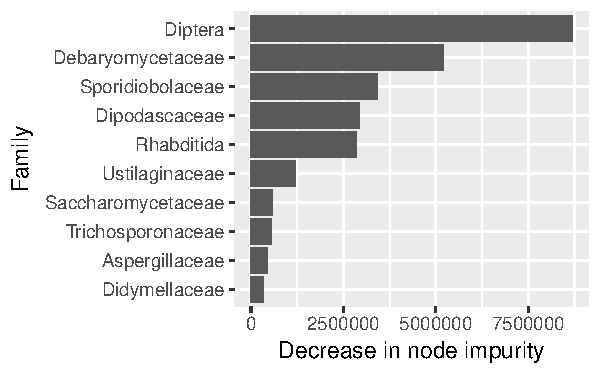
\includegraphics{../../../eukaryote_data/only_families/all_time_steps/hit_1perc_twice/orig_units_all_data_families_barchart}
  \caption{Most influential eukaryote family-level taxa}
  \label{fig:infl_eukaryote_family_taxa}
\end{figure}

\begin{figure}
  \centering
  \includegraphics{../../../eukaryote_data/only_families/all_time_steps/influential_family_taxa_panel}
  \caption{Some of the influential eukaryote family-level taxa, by degree day}
  \label{fig:scatter_eukaryote_family_taxa}
\end{figure}

Figure \ref{fig:resids_cv_eukaryote_family_taxa} shows a scatterplot
of the errors vs.~the actual degree days, across all 1000
cross-validation runs.  The pattern is much the same as those
identified in the earlier sections, using Shane's data.  In a
real-world application, though, we may not have any observations
corresponding to the actual degree days accumulated post mortem.
Figure \ref{fig:leave_one_out_resids_eukaryote_family_taxa} shows
these residuals, which again show patterns similar to those seen in
earlier sections.  The root mean squared estimation error in these
cases is about 243.6, which is better than that using the
bacteria-only dataset.
%% The RMSE for predictions of left-out individuals on days where we do
%% have data is about 186.2.

\begin{figure}
  \centering
  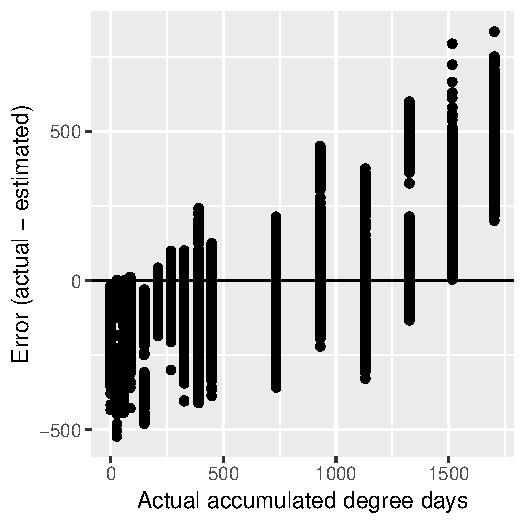
\includegraphics{../../../eukaryote_data/only_families/all_time_steps/hit_1perc_twice/orig_units_all_data_families_residuals}
  \caption{Residuals from the cross-validation runs for the eukaryote family-level taxa model}
  \label{fig:resids_cv_eukaryote_family_taxa}
\end{figure}

\begin{figure}
  \centering
  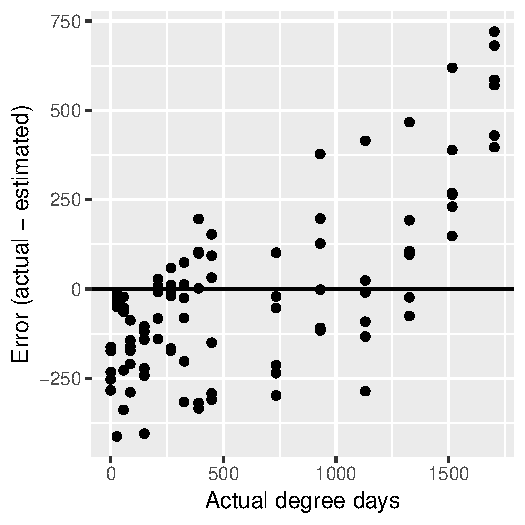
\includegraphics{../../../eukaryote_data/only_families/all_time_steps/hit_1perc_twice/leave_out_one_subj_and_one_day_residuals}
  \caption{Residuals for model runs leaving out one subject and one day (eukaryote family-level taxa)}
  \label{fig:leave_one_out_resids_eukaryote_family_taxa}
\end{figure}


\subsubsection{Results for order-level taxa}

Table \ref{tbl:eukaryote_order_all_data_model_stats} shows the model
performance statistics for the eukaryote order-level taxa, which again
seems to indicated a better fit than the model for the same level taxa
in Shane's dataset.  Figures \ref{fig:infl_eukaryote_order_taxa} and
\ref{fig:scatter_eukaryote_order_taxa} show some of the influential
order-level taxa.

\begin{table}
  \centering
\caption{\label{tbl:eukaryote_order_all_data_model_stats}Model statistics using order-level eukaryote taxa}
\begin{tabular}{llll}
Inclusion cutoff & Units  & RMSE & Explained variation\\ \hline
1\% at least twice (stricter) & Orig.~units & 193.2 & 87.67\% 
\end{tabular}
\end{table}

\begin{figure}
  \centering
  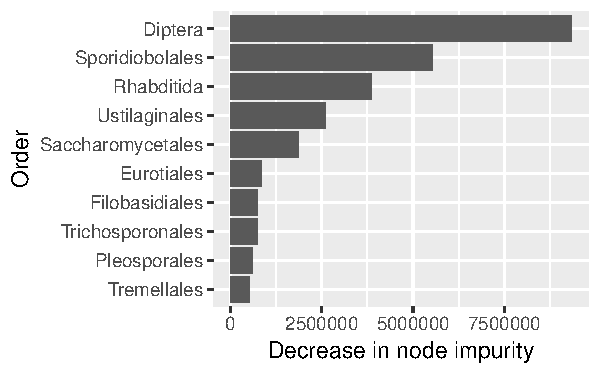
\includegraphics{../../../eukaryote_data/only_orders/all_time_steps/hit_1perc_twice/orig_units_all_data_orders_barchart}
  \caption{Most influential eukaryote order-level taxa}
  \label{fig:infl_eukaryote_order_taxa}
\end{figure}

\begin{figure}
  \centering
  \includegraphics{../../../eukaryote_data/only_orders/all_time_steps/influential_order_taxa_panel}
  \caption{Some of the influential eukaryote order-level taxa, by degree day}
  \label{fig:scatter_eukaryote_order_taxa}
\end{figure}



\subsection{Models using only the first 15 days of data}

\subsubsection{Results for family-level taxa}

The model performance statistics are shown in Table
\ref{tbl:eukaryote_family_first_15days_model_stats}.  These seems to
indicate a better fit than using the bacteria-only dataset shown in
the previous section.

\begin{table}
  \centering
\caption{\label{tbl:eukaryote_family_first_15days_model_stats}Model statistics using family-level eukaryote taxa}
\begin{tabular}{llll}
Inclusion cutoff & Units  & RMSE & Explained variation\\ \hline
1\% at least twice (stricter) & Orig.~units & 58.6 & 84.65\% 
\end{tabular}
\end{table}

Figures \ref{fig:infl_eukaryote_family_taxa_first_15days} and
\ref{fig:scatter_eukaryote_family_taxa_first_15days} show a few of the
family taxa which the model showed to be influential when modeling
just the first 15 days.

\begin{figure}
  \centering
  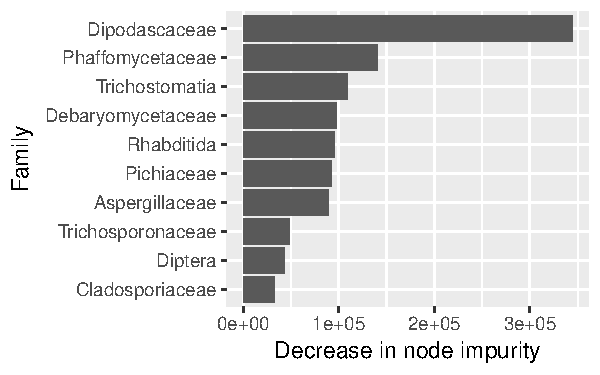
\includegraphics{../../../eukaryote_data/only_families/first_two_weeks/hit_1perc_twice/orig_units_first_two_weeks_families_barchart}
  \caption{Most influential eukaryote family-level taxa, first 15 days}
  \label{fig:infl_eukaryote_family_taxa_first_15days}
\end{figure}

\begin{figure}
  \centering
  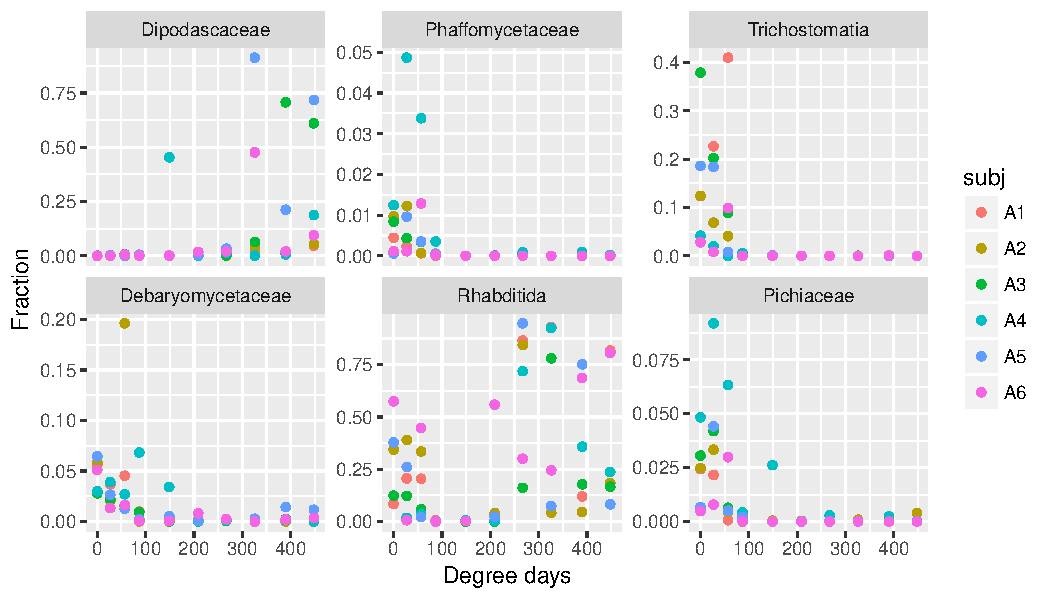
\includegraphics{../../../eukaryote_data/only_families/first_two_weeks/influential_family_taxa_panel_first_two_weeks}
  \caption{Some of the influential eukaryote family-level taxa, by degree day (first 15 days)}
  \label{fig:scatter_eukaryote_family_taxa_first_15days}
\end{figure}

Figure \ref{fig:leave_one_out_resids_eukaryote_family_taxa_first_15days}
shows a plot of the model residuals for our simulations of cases in
which we leave out all the observations from one day and one subject,
and try to predict the missing day and subject.  The pattern is
similar to that seen in previous, similar plots.  The RMSE for
predictions in these cases is about 93.4.

\begin{figure}
  \centering
  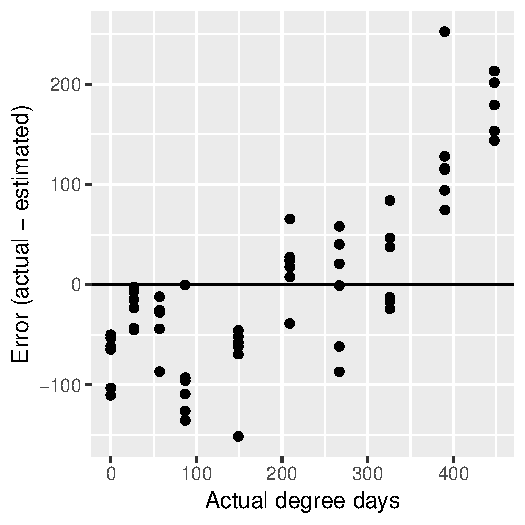
\includegraphics{../../../eukaryote_data/only_families/first_two_weeks/hit_1perc_twice/leave_out_one_subj_and_one_day_residuals}
  \caption{Residuals for model runs leaving out one subject and one day (eukaryote family-level taxa, first15 days)}
  \label{fig:leave_one_out_resids_eukaryote_family_taxa_first_15days}
\end{figure}




\section{References}

\noindent James, G., Witten, D., Hastie, T., Tibshirani, R. (2013) \textit{An
  Introduction to Statistical Learning with Applications in R}. New
York: Springer

\noindent Metcalf, J. L., et al. (2016).  Microbial community assembly and
metabolic function during mammalian corpse decomposition.
\textit{Science}, Vol.~351, 158-162.

\end{document}

